\chapter{Constructions}

\section{Introduction}

In this chapter, we present diagrammed proofs of lethal sets that percolate at the lower bound. The proofs are organized by the thickness of the grid. Many of the constructions in the following sections belong to infinite families of either optimal or perfect sets. In this case, we shall examine the grids by region, and observe that certain regions can be expanded to arbitrarily large sizes using mathematical induction. 

We shall call a thickness \emph{semi-complete} if all divisibility cases are optimal.

\section{Useful lemmas and observations}

We shall see that similar patterns and structures appear with some regularity in optimal sets. These structures always infect entire regions, and it will be helpful to recognize them within larger grids when they appear. 

\begin{lem}
\label{lem:forest}
Let $G = P_a \Osq P_b$ be a graph and $S \subseteq V(G)$ be a subset of the vertices of $G$. Let $G[\overline{S}]$ be the subgraph of $G$ induced by vertices not in $S$. Then $S$ is a lethal set if and only if $G[\overline{S}]$ is cycle-free, and has no paths between any two boundary vertices. 
\end{lem}

\begin{lem}
\label{lem:three_walls}
Let $G$ be a rectangular prism $(a,b,c)$. If a set $S$ is lethal on three mutually orthogonal faces of $G$, then $S$ is lethal on $G$.
\end{lem}

\begin{cor}
\label{cor:three_walls}
Let $G$ be a grid assembled from sub-grids $G_1, \dots, G_k$. Let $H_1, \dots, H_k$ be sets satisfying the conditions of lemma \ref{lem:three_walls} for sub-grids $G_1, \dots, G_k$, respectively. Then $H = H_1 \cup \dots \cup H_k$ is a lethal set in $G$.
\end{cor}

%\begin{lem}
%\label{lem:unfold}
%Let $G$ be the grid $(a,b,c)$. Let $H$ be a subgraph induced by the vertices of $G$. If the projection of $H$ in the $x$ direction gives the graph $(b,c)$, in the $y$ direction gives $(a,c)$, and in the $z$ direction gives $(a,b)$, and $H$ percolates, then $G$ percolates.
%\end{lem}

%\begin{proof}
%The projection condition guarantees that $G$ has lethal sets on three perpendicular planes. The result follows from lemma \ref{lem:three_walls}.
%\end{proof}

We refer to the union of mutually orthogonal faces of sub-grids $G_1, \dots, G_k$ as a \emph{manifold} of $G$. Therefore, corollary \ref{cor:three_walls} says that if a set $H$ is lethal on the manifold of $G$, then $H$ is lethal in $G$. Furthermore, we define a \emph{proper unfolding} of $G$ as a planar representation of the manifold of $G$. This can be thought of as a special type of folding net of $G$, such that when assembled the resulting structure satisfies the conditions of corollary \ref{cor:three_walls}. 

%\begin{cor}
%\label{cor:unfold}
%Something about unfolding $H$ and its planar embedding. Imagine $H$ as a set of folded up pieces of paper. Let $\mathcal{N}$ be the family of unfolded nets comprising $H$. To show that $G$ percolates, it is sufficient to show that all nets $N \in \mathcal{N}$ harbor lethal infections.
%\end{cor}

\section{Thickness 1}

There are two general constructions in thickness 1 that percolate at the surface area bound. The first construction is perfect for all $(2^n-1, 2^n-1, 1)$ grids, and originates in a 2021 paper by Benevides et al. \cite{benevides:2021}. The second construction is optimal for all grids $(a,b,1)$, where $a \equiv 5 \pmod 6$, $b \equiv 1 \pmod 2$, and $a,b \geq 5$. As such grids constitute non-divisibility cases, this construction is not perfect.

% Purina constructions that percolate at the S.A. bound
\subsection{Purina}

We refer to this construction colloquially as the Purina construction, due to the similarly between its instance on the $(3,3,1)$ grid and the logo of the pet food brand. No funding has been offered, but we are open to the possibility. A more extensive discussion on this pattern can be found in \cite{benevides:2021}.

\begin{con}
\label{con:purina}
All grids of the form $(2^n-1, 2^n-1, 1)$ are perfect.
\end{con}

\begin{figure}[]
\centering
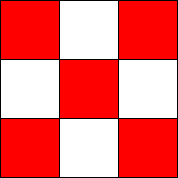
\includegraphics[width=0.1\textwidth]{figures/4/3x3x1.pdf}
\caption{A perfect percolating set for $(3,3,1)$.}
\label{fig:3x3x1}
\end{figure} 

\begin{proof}
This is a recursive construction built from the base component piece shown in figure \ref{fig:3x3x1}. Note that this $(3,3,1)$ construction is lethal under the 3-neighbor bootstrap process, and that it meets the surface area bound:
$$\frac{1}{3} \cdot (ab+bc+ca) = \frac{1}{3} \cdot (9 + 3 + 3) = 5.$$
For larger grids of size $(2^n-1, 2^n-1, 1)$, join four copies of $(2^{n-1}-1, 2^{n-1}, 1)$ about two perpendicular corridors, and infect the vertex at their intersection (figure \ref{fig:15x15x1}). Observe that the resulting set is lethal: each of the four smaller grids is lethal by hypothesis, and the remaining vertices induce a forest with disconnected boundary points, which percolates by lemma \ref{lem:forest}. Furthermore, note that
\begin{align*}
\text{S.A.}(2^n-1,2^n-1,1) &= \frac{1}{3} \cdot (2^{2n}-1) \\
&= 4 \cdot \frac{1}{3} \cdot (2^{2n-2} -1) + 1 = 4 \cdot \text{S.A.}(2^{n-1}-1, 2^{n-1}, 1) + 1,
\end{align*}
and therefore this construction is perfect.
\end{proof}

\begin{figure}[]
\centering
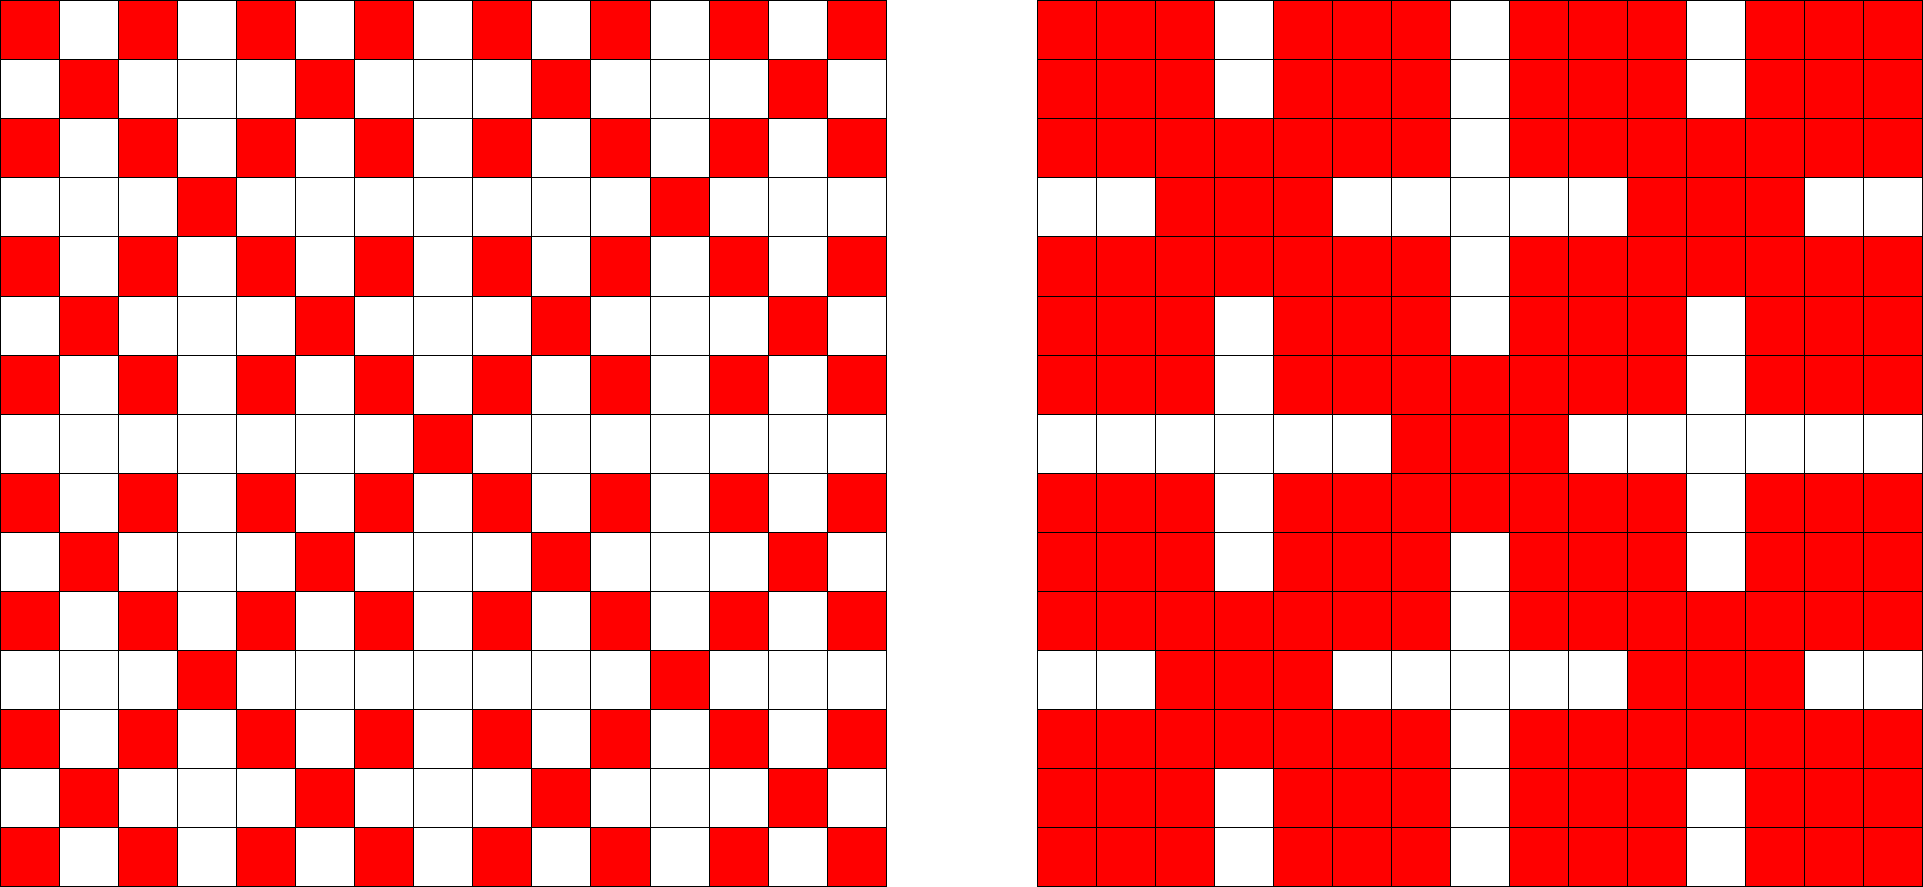
\includegraphics[width=0.6\textwidth]{figures/4/15x15x1.pdf}
\caption{A perfect percolating set for $(15,15,1)$.}
\label{fig:15x15x1}
\end{figure} 

% (odd)x(odd) constructions that percolate at the S.A. bound
\subsection{Snakes}

As indicated by lemma \ref{lem:forest}, a fundamental characteristic of lethal sets $S$ is the presence of an initially uninfected corridor, bounded by walls of infection. This structure is apparent in the second diagrams of figures \ref{fig:15x15x1} and \ref{fig:11x13x1}. These corridors correspond to forests in the complement $G[\overline{S}]$ of $S$. In this subsection, we provide a general method for constructing such corridors in $(a, b, 1)$ grids where $a \equiv 5 \pmod 6$ and $b \equiv 1 \pmod 2$.

% WITH THE EXCEPTION OF WIDTH 3!!!!!
% WIDTH >= 5
\begin{con}
\label{con:snake}
All grids of the form $(a,b,1)$, $a \equiv 5 \pmod 6$, $b \equiv 1 \pmod 2$, and $a,b \geq 5$ are optimal.
\end{con}

\begin{proof}
For grids of the form $(a,b,1)$, $a \equiv 5 \pmod 6$, $b \equiv 1 \pmod 2$, we construct an optimal infected set and show that it percolates by lemma \ref{lem:forest}. For the base case, consider the $(5,5,1)$ grid $G$ illustrated in figure \ref{fig:5x5x1}. Observe that this construction is optimal. Now consider the grid $G'$ resulting from the insertion of a $(5, 2k, 1)$ block, as shown in figure \ref{fig:5x13x1}. Note that the subgraph induced by the uninfected vertices of $G'$ satisfies the conditions of lemma \ref{lem:forest}. Furthermore, note that if any $(5, n, 1)$ grid is optimal, the $(5,n+2,1)$ grid resulting from such a construction has surface area bound $\text{S.A.}(5,n,1) + 4$, which agrees with the number of infected vertices.

\begin{figure}[]
\centering
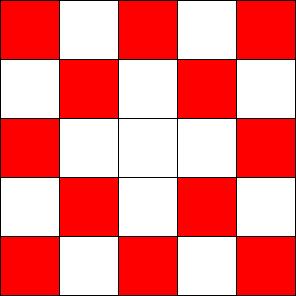
\includegraphics[width=0.15\textwidth]{figures/4/5x5x1.pdf}
\caption{An optimal percolating set for $(5,5,1)$.}
\label{fig:5x5x1}
\end{figure} 

\begin{figure}[]
\centering
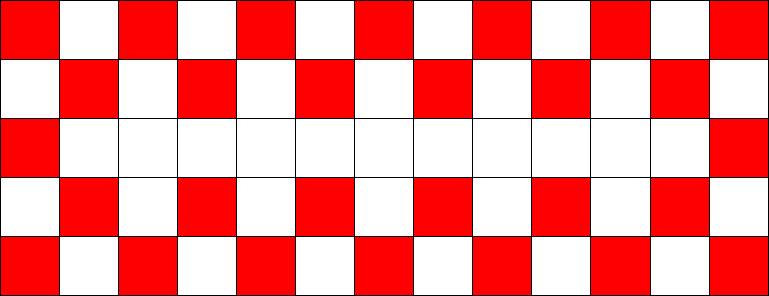
\includegraphics[width=0.5\textwidth]{figures/4/5x13x1.pdf}
\caption{An optimal percolating set for $(5,13,1)$.}
\label{fig:5x13x1}
\end{figure} 

To extend this construction in the vertical direction, we introduce a kink in the snaking infection. This kink requires six rows to produce a repeating pattern. The structure of this design is shown in figure \ref{fig:11x13x1}. For grids of smaller width, the same construction gives optimal percolating sets; however, the snaking pattern is increasingly difficult to recognize in thin grids.
\end{proof}

\begin{figure}[]
\centering
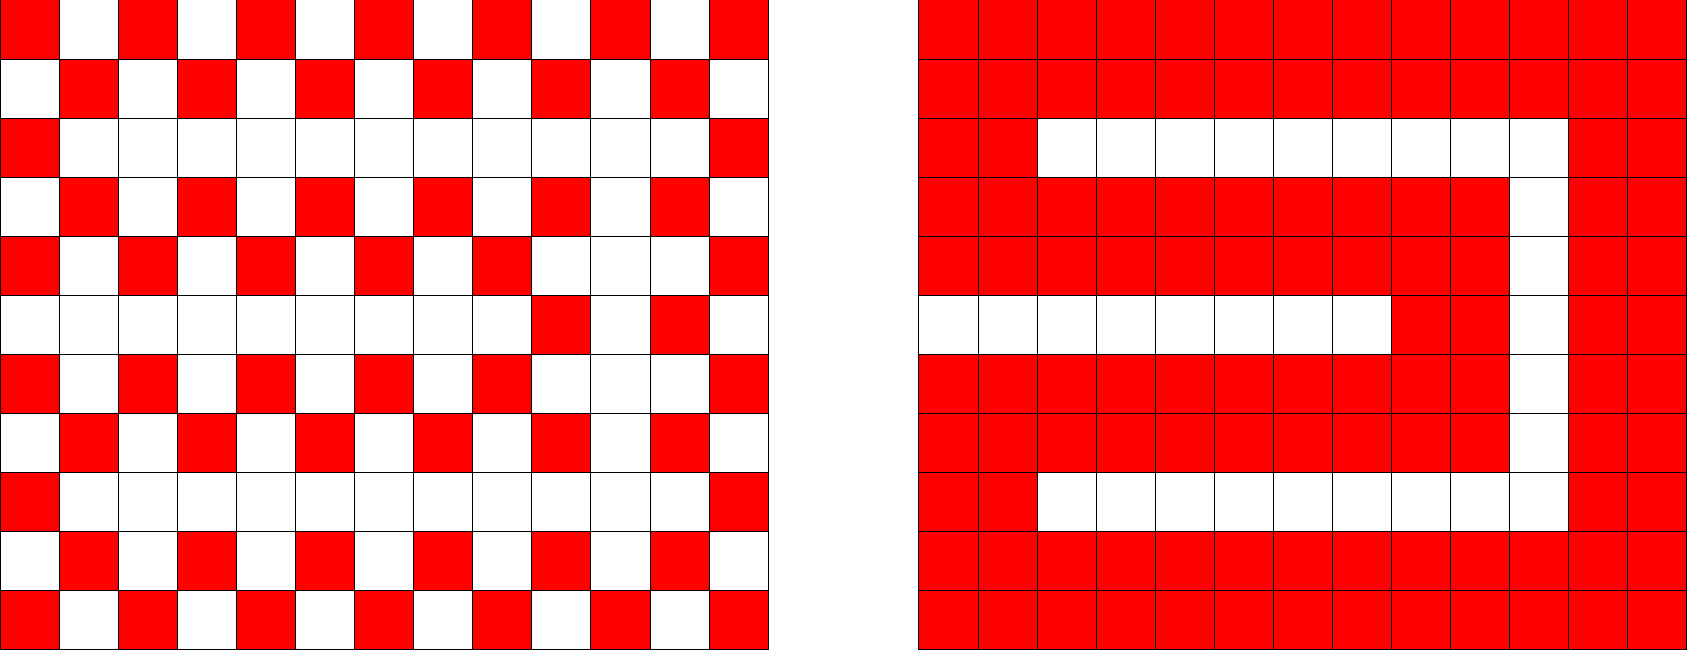
\includegraphics[width=0.6\textwidth]{figures/4/11x13x1.pdf}
\caption{An optimal percolating set for $(11,13,1)$.}
\label{fig:11x13x1}
\end{figure} 

% Maybe other (divisibility) constructions that percolate at 1 over the bound (if they exist)?

\section{Thickness 2}

In this section we examine four infinite families of perfect grids. We show that each has a manifold that admits a lethal set of perfect size. We note that such lethal sets are likely to exist for nearly all divisibility cases in thickness two; however, constructions are elusive and those presented here are sufficient to prove the main result of this thesis.

% (0 mod 6, 3, 2)
\begin{con}
All $(a,3,2)$ grids with $a \equiv 0 \pmod 6$ are perfect. 
\end{con}

\begin{figure}[]
\centering
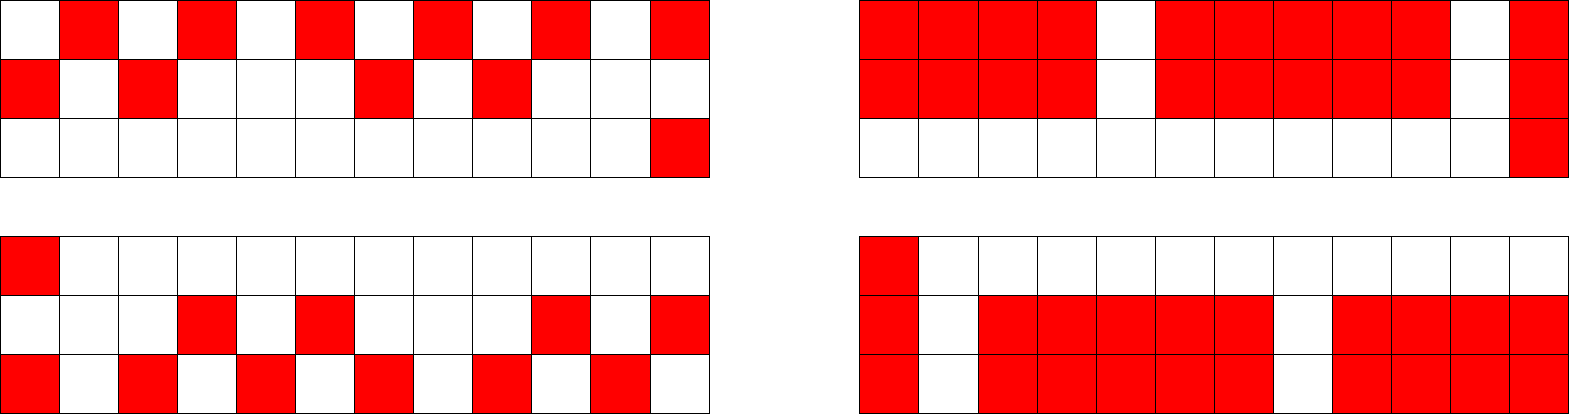
\includegraphics[width=0.8\textwidth]{figures/4/3x12x2.pdf}
\caption{A perfect percolating set for $(3,12,2)$.}
\label{fig:3x12x2}
\end{figure} 

\begin{figure}[]
\centering
%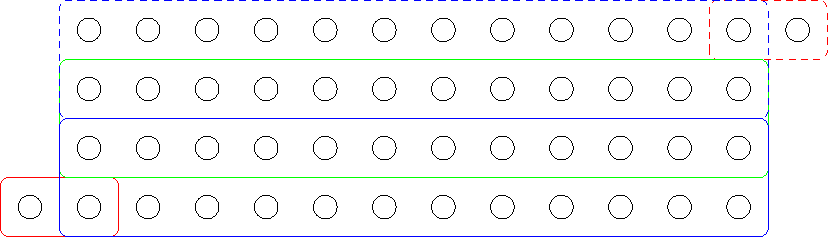
\includegraphics[width=0.6\textwidth]{figures/4/3x12x2_manifold.pdf}
\caption{A proper unfolding of $G= (3,12,2)$. Colored rectangles indicate faces of $G$. Dashed lines indicate that cells appear on different layers. }
\label{fig:3x12x2_manifold}
\end{figure} 

\begin{figure}[]
\centering
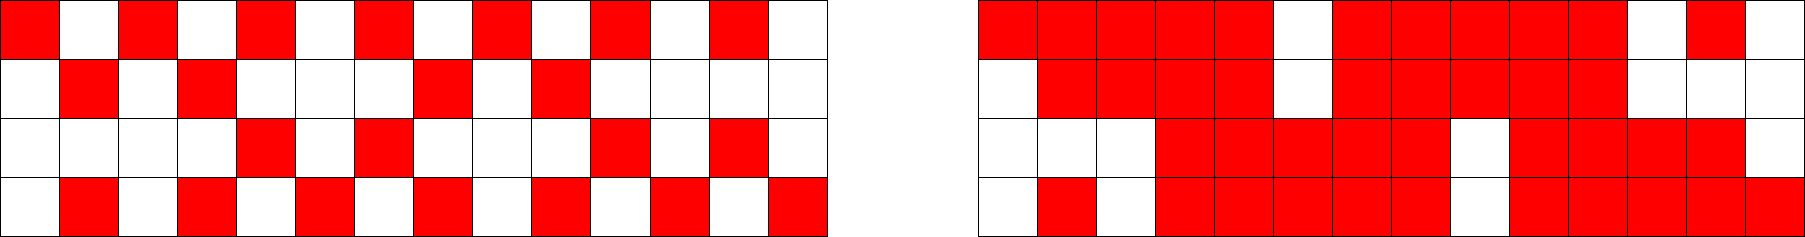
\includegraphics[width=0.8\textwidth]{figures/4/3x12x2_unfolded_lethal.pdf}
\caption{A percolating set on the proper unfolding of $G= (3,12,2)$.}
\label{fig:3x12x2_unfolded_lethal}
\end{figure} 

\begin{proof}
\end{proof}

% (3 mod 6, 3, 2)
\begin{con}
All $(a,3,2)$ grids with $a \equiv 0 \pmod 6$ are perfect. 
\end{con}

\begin{proof}
\end{proof}

% (2 mod 6, 5 mod 6, 2)

% a,b, MUST BE A CERTAIN SIZE
\begin{con}
All $(a,b,2)$ grids with $a,b \in \{2,5\} \pmod 6$ and $a \neq b \pmod 6$ are perfect. 
\end{con}

\begin{figure}[]
\centering
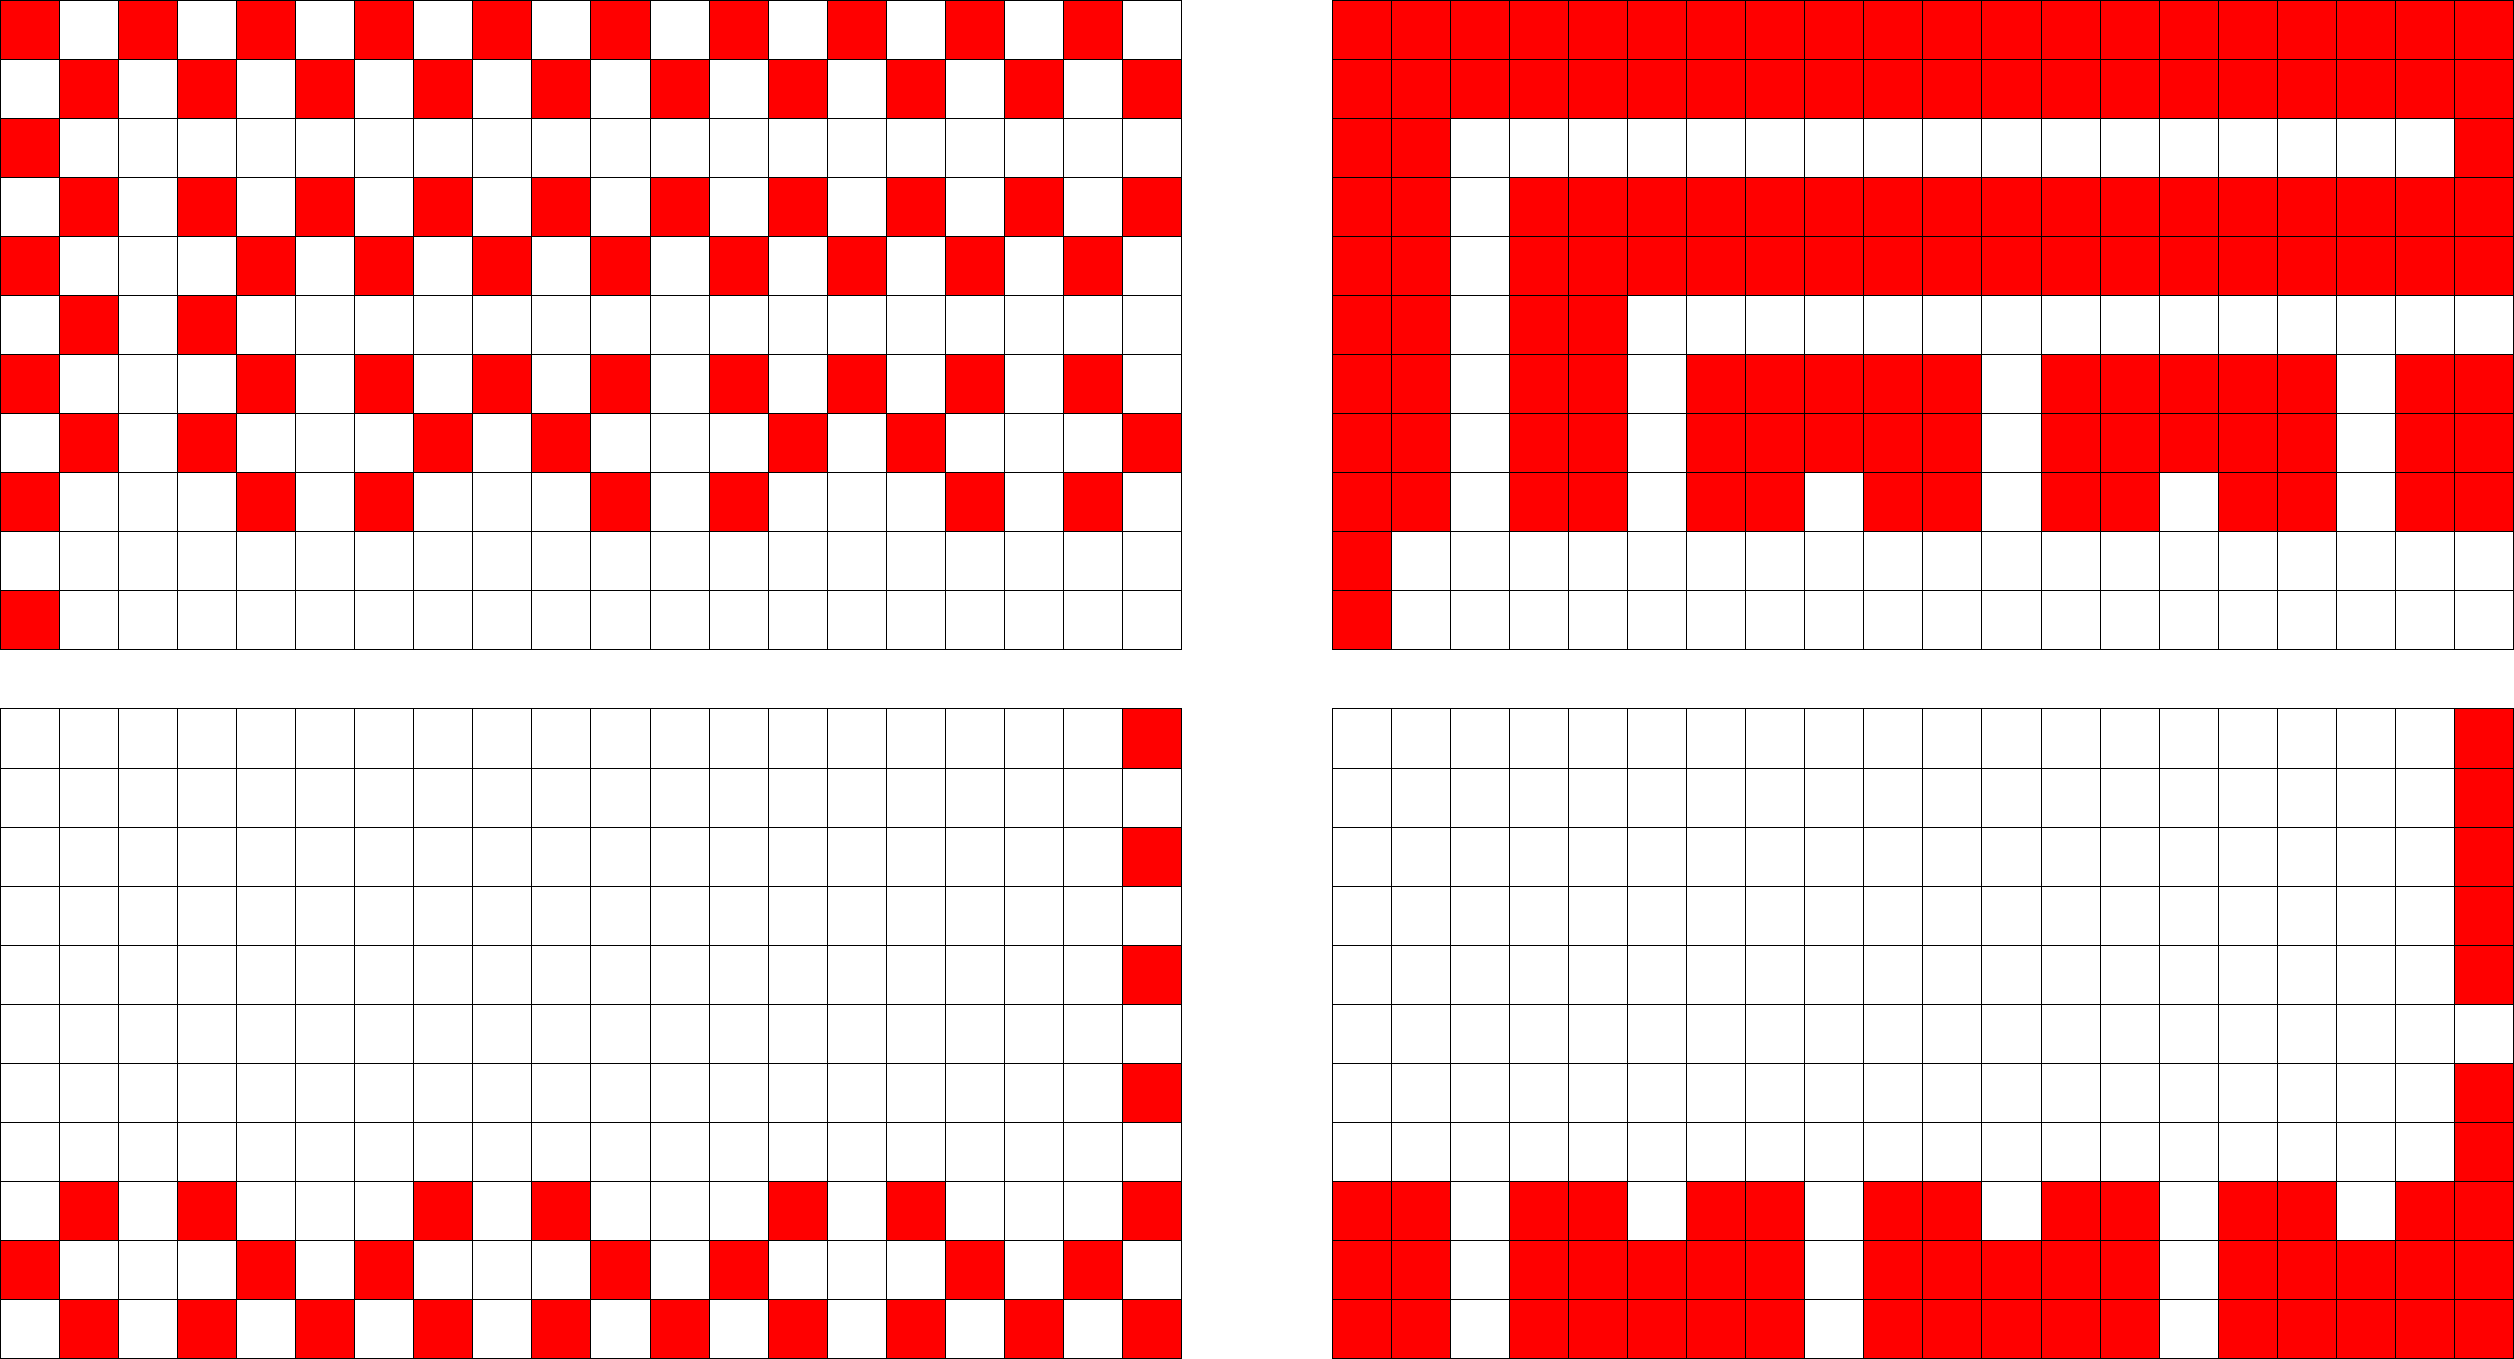
\includegraphics[width=0.8\textwidth]{figures/4/11x20x2.pdf}
\caption{A perfect percolating set for $(11,20,2)$.}
\label{fig:11x20x2}
\end{figure} 

\begin{figure}[]
\centering
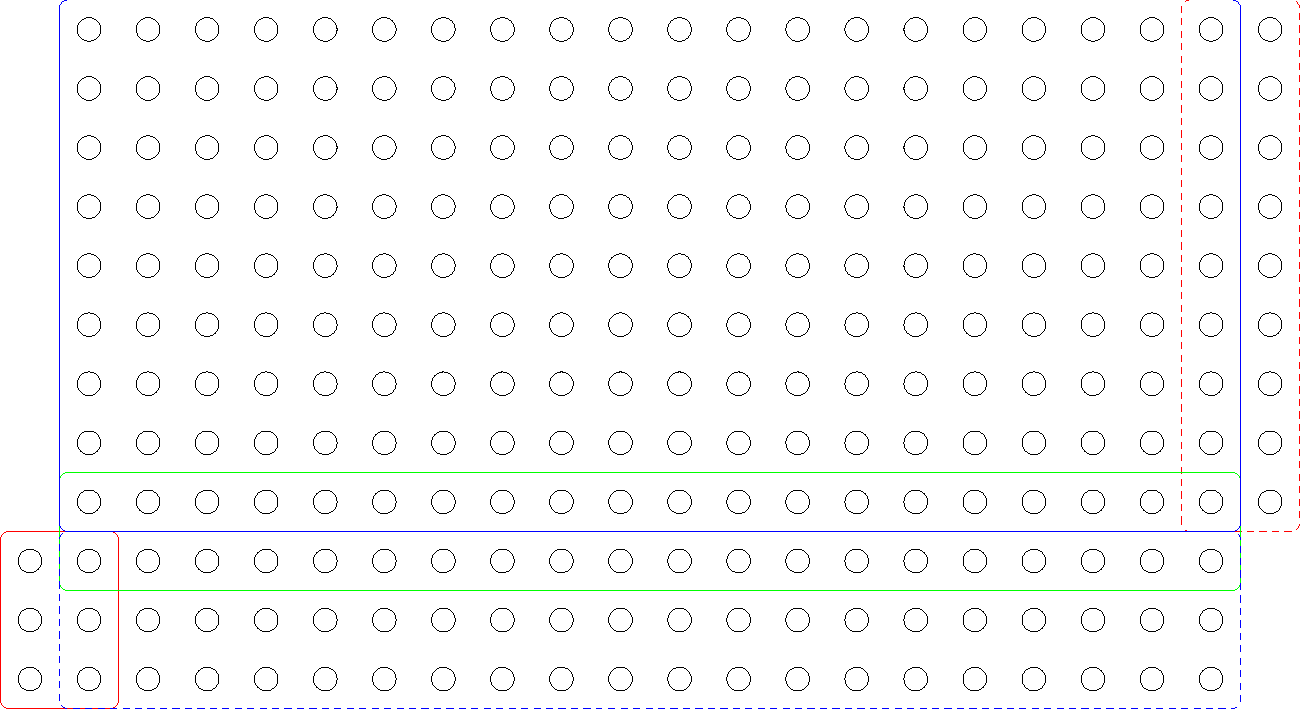
\includegraphics[width=0.6\textwidth]{figures/4/11x20x2_manifold.pdf}
\caption{A proper unfolding of $G= (11,20,2)$. Colored rectangles indicate faces of $G$. Dashed lines indicate that cells appear on different layers. }
\label{fig:11x20x2_manifold}
\end{figure} 

\begin{figure}[]
\centering
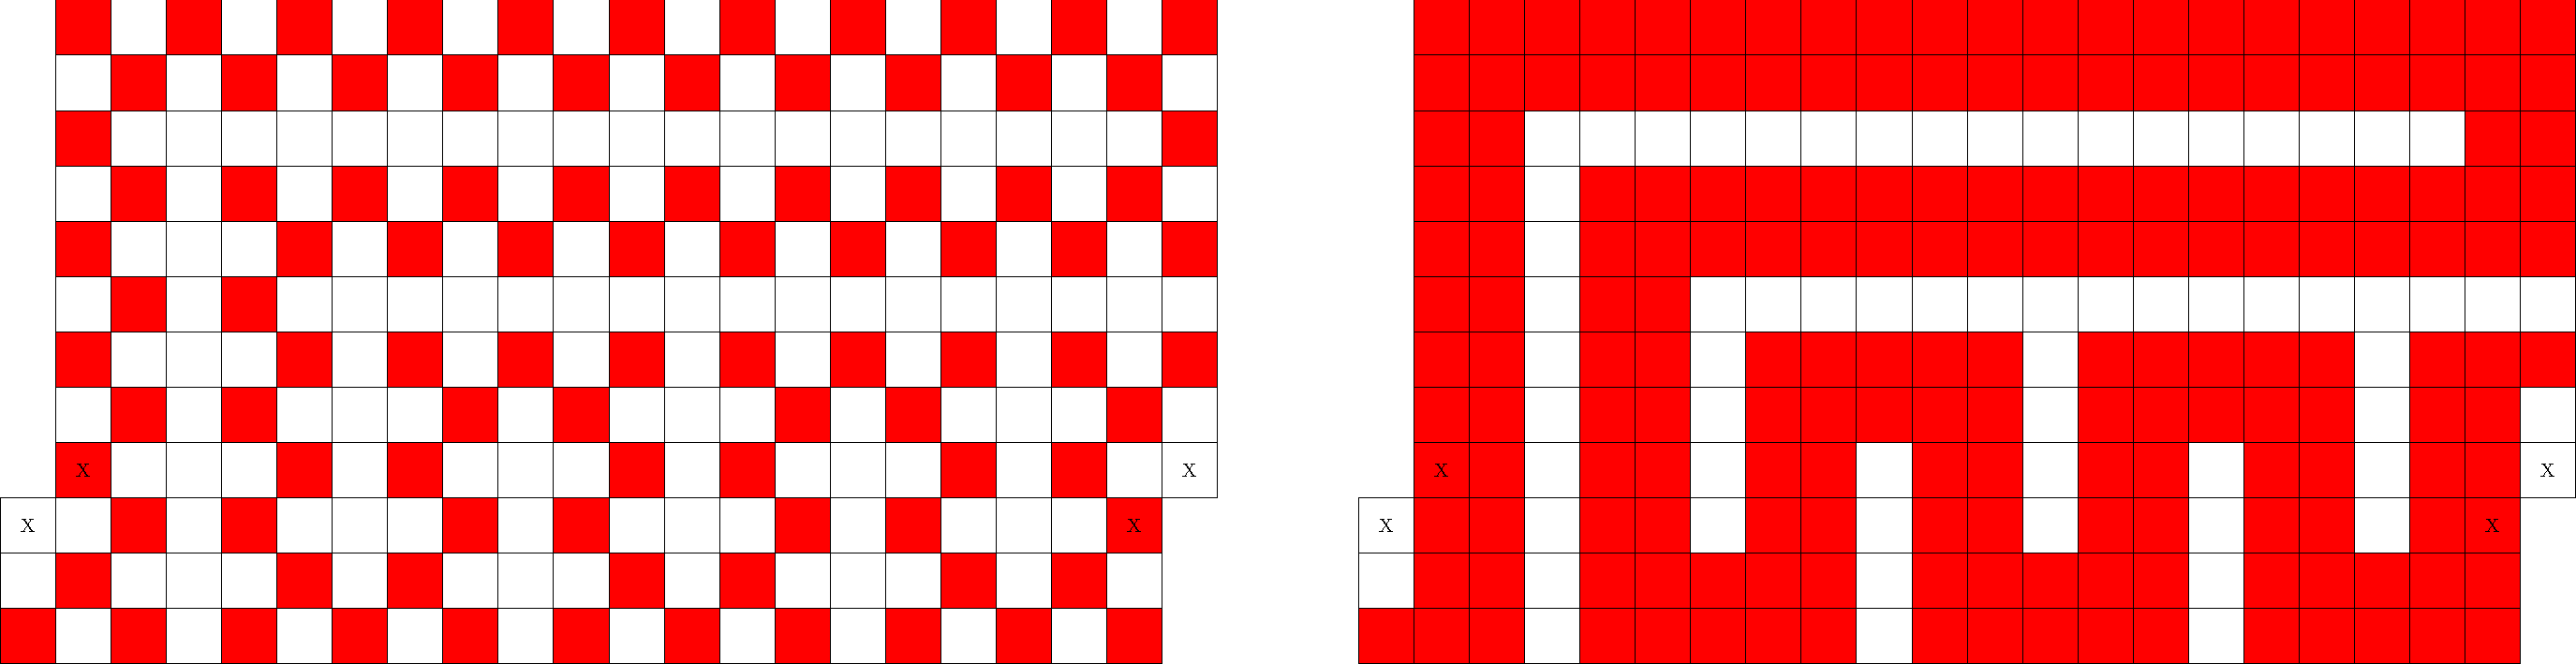
\includegraphics[width=0.8\textwidth]{figures/4/11x20x2_unfolded_lethal.pdf}
\caption{A percolating set on the proper unfolding of $G= (11,20,2)$.}
\label{fig:11x20x2_unfolded_lethal}
\end{figure} 

\begin{proof}
Let $G$ be an $(a,b,2)$ grid with $a,b \in \{2,5\} \pmod 6$ and $a \neq b \pmod 6$, and let $H$ be an unfolding of $G$ (figure \ref{fig:11x20x2_manifold}). We show that this unfolding is proper, and that it admits a perfect lethal set. 

The above construction holds for $a \geq 11$ and $b \geq 8$. SAY SOMETHING ABOUT THE MISSING CASES.
\end{proof}

% (3 mod 6, 0 mod 6, 2) 

% a,b MUST BE A CERTAIN SIZE
\begin{con}
All $(a,b,2)$ grids with $a,b \in \{0,3\} \pmod 6$ and $a \neq b \pmod 6$ are perfect. 
\end{con}

\begin{proof}
Consider the $(21,12,2)$ grid $G$ shown in figure \ref{fig:12x21x2}. Let $H$ be a unfolding of $G$ (figure \ref{fig:12x21x2_unfolded}). Observe that $H$ is proper: three mutually orthogonal faces of $G_1$ are shown by blue, green and dashed red regions, and mutually orthogonal faces of $G_2$ are shown by the red, green and dashed blue regions. We show that $H$ admits a lethal set of size $\text{S.A.}(12,21,2) = 106$. Consider such a set, as shown in figure \ref{fig:12x21x2_unfolded_lethal}. (Observe that this is the same set as shown in figure \ref{fig:12x21x2}.) By lemma \ref{lem:forest}, this set percolates with the exception of two $C_4$s in the top and bottom of the grid. However, notice that one of these cells is a duplicate of an already infected cell. (This duplication is a consequence of the proper unfolding of $G$.) Therefore, $H$ admits a lethal set, and by corollary \ref{cor:three_walls}, $G$ is perfect.

For all larger grids, observe that the snaking corridor in the left side $G$ can be extended by multiples of 6 in both the $x$ and $y$ directions. These resulting grid still percolates under lemma \ref{lem:forest}. A simple calculation verifies that such an alteration produces initial infections at the surface area bound. 
\end{proof}

\begin{figure}[]
\centering
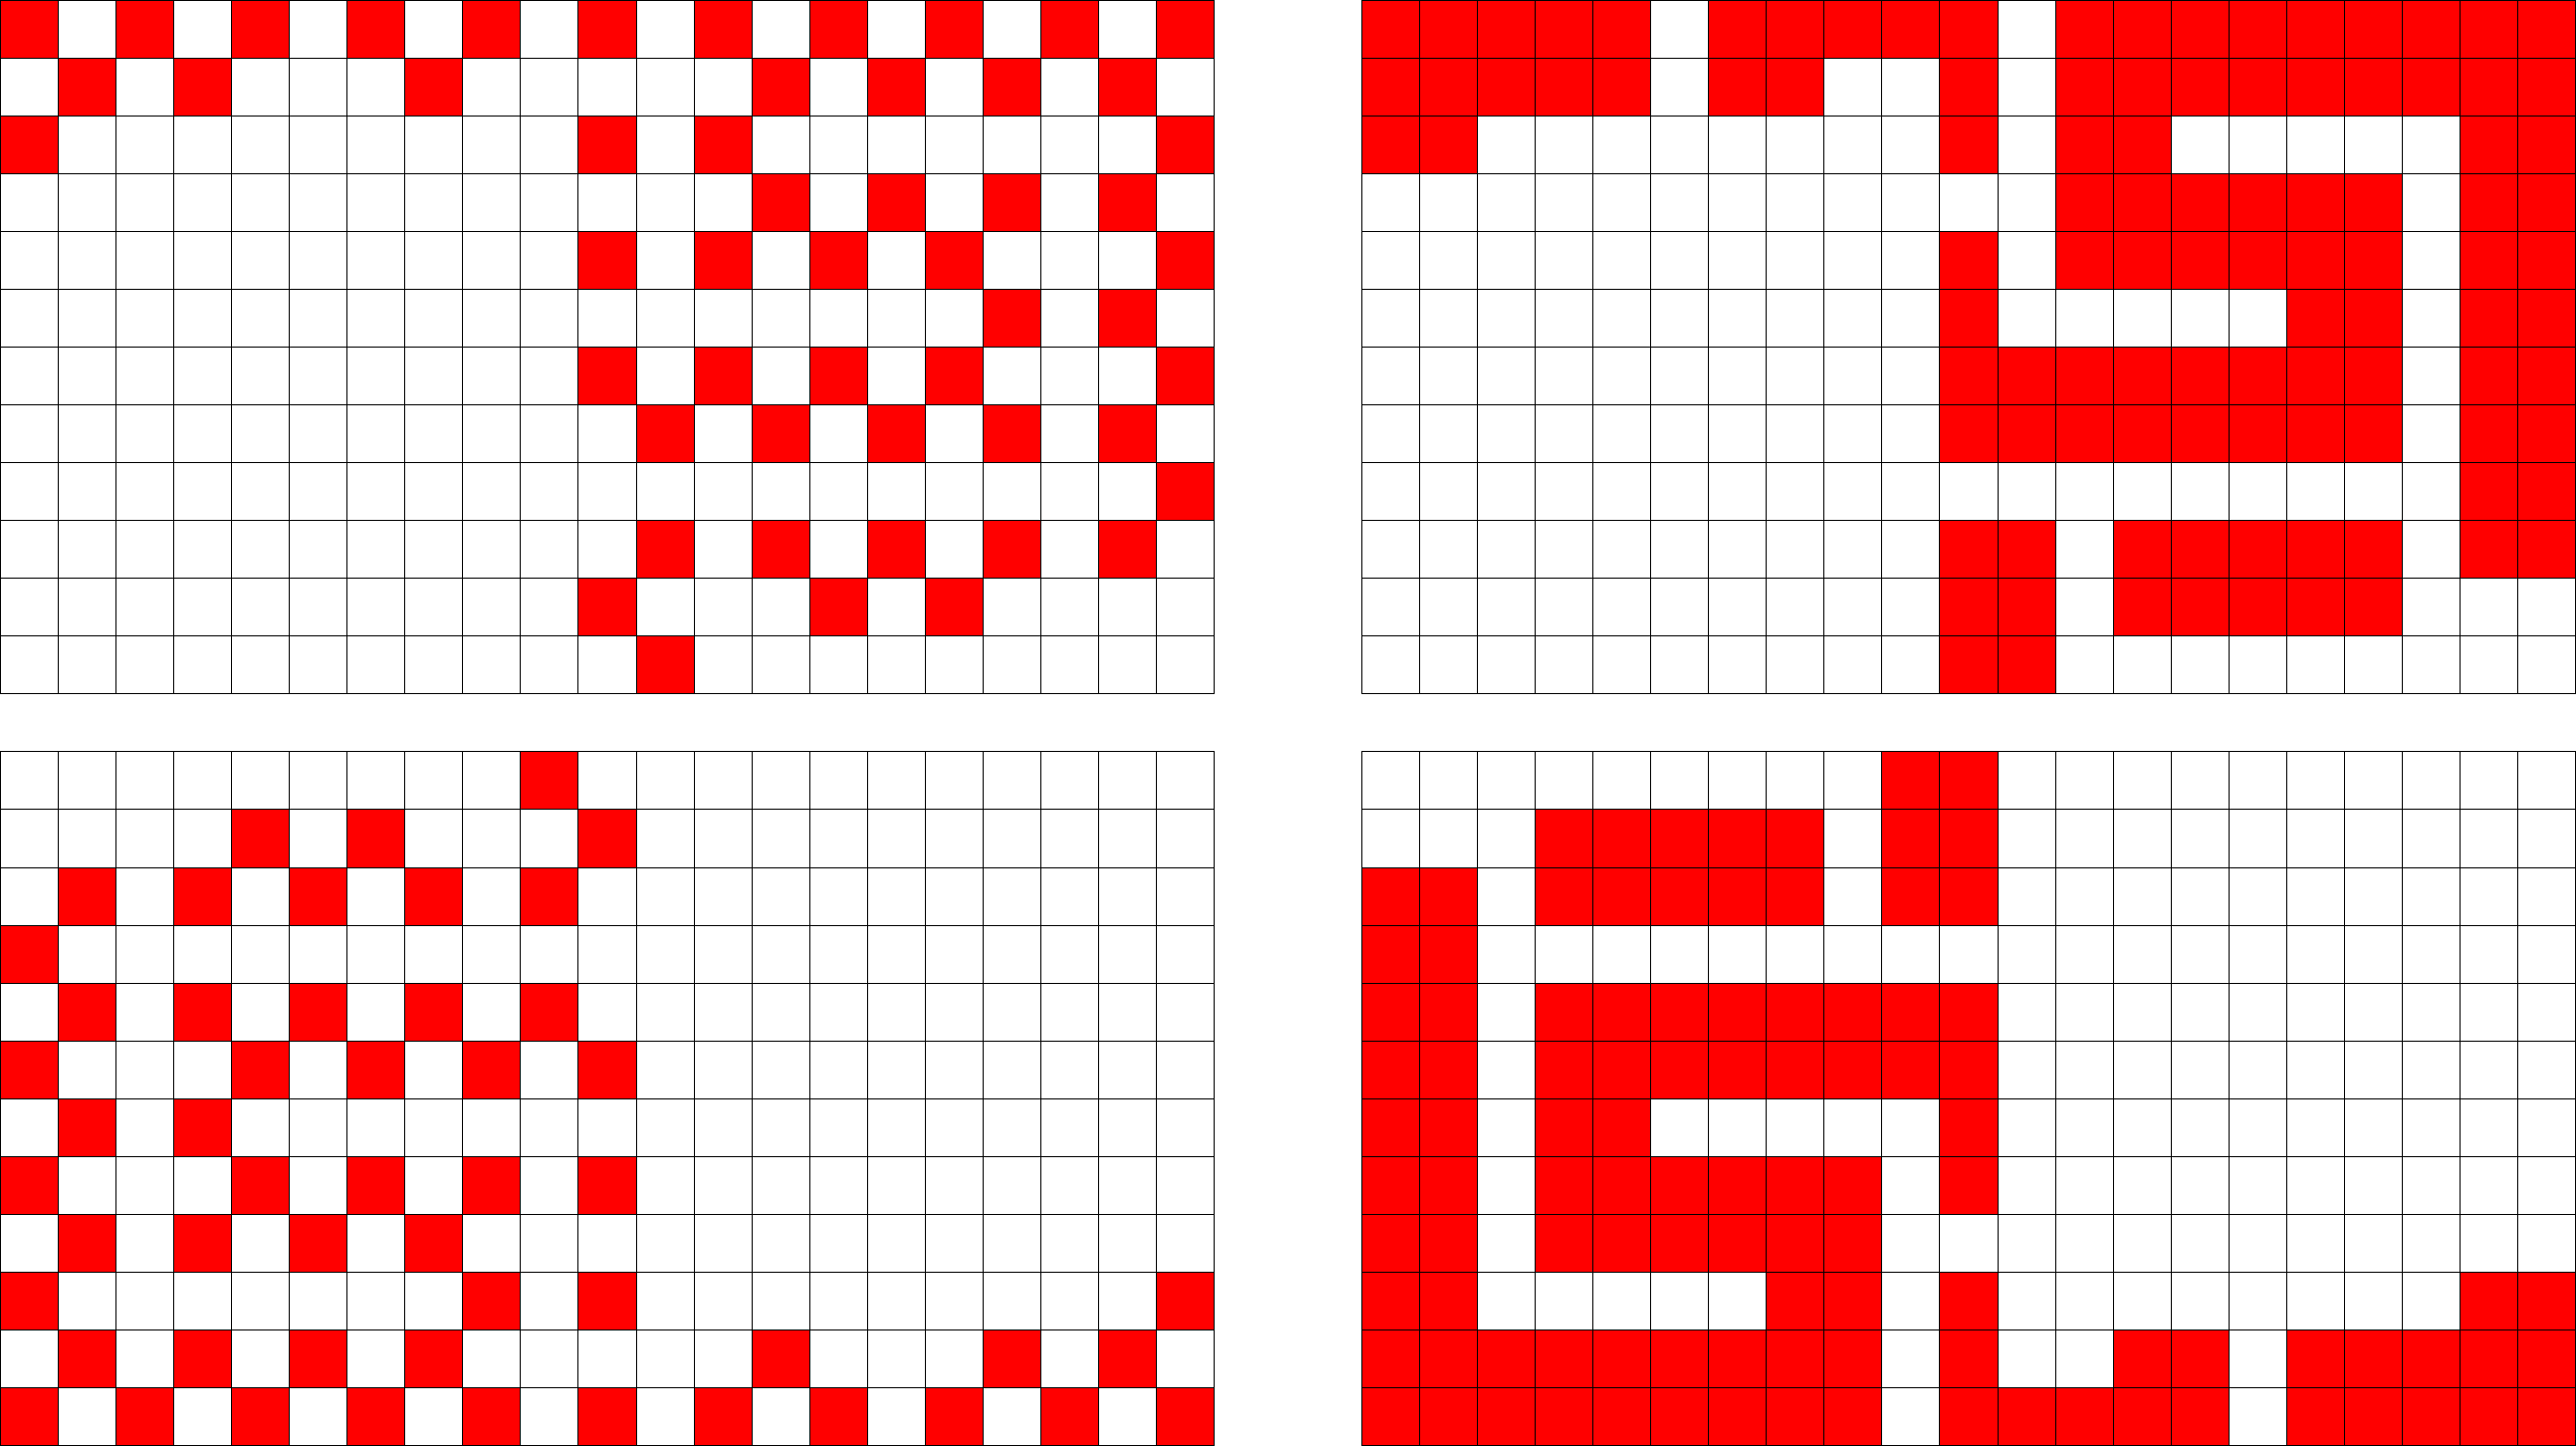
\includegraphics[width=0.8\textwidth]{figures/4/12x21x2.pdf}
\caption{A perfect percolating set for $(12,21,2)$.}
\label{fig:12x21x2}
\end{figure} 

\begin{figure}[]
\centering
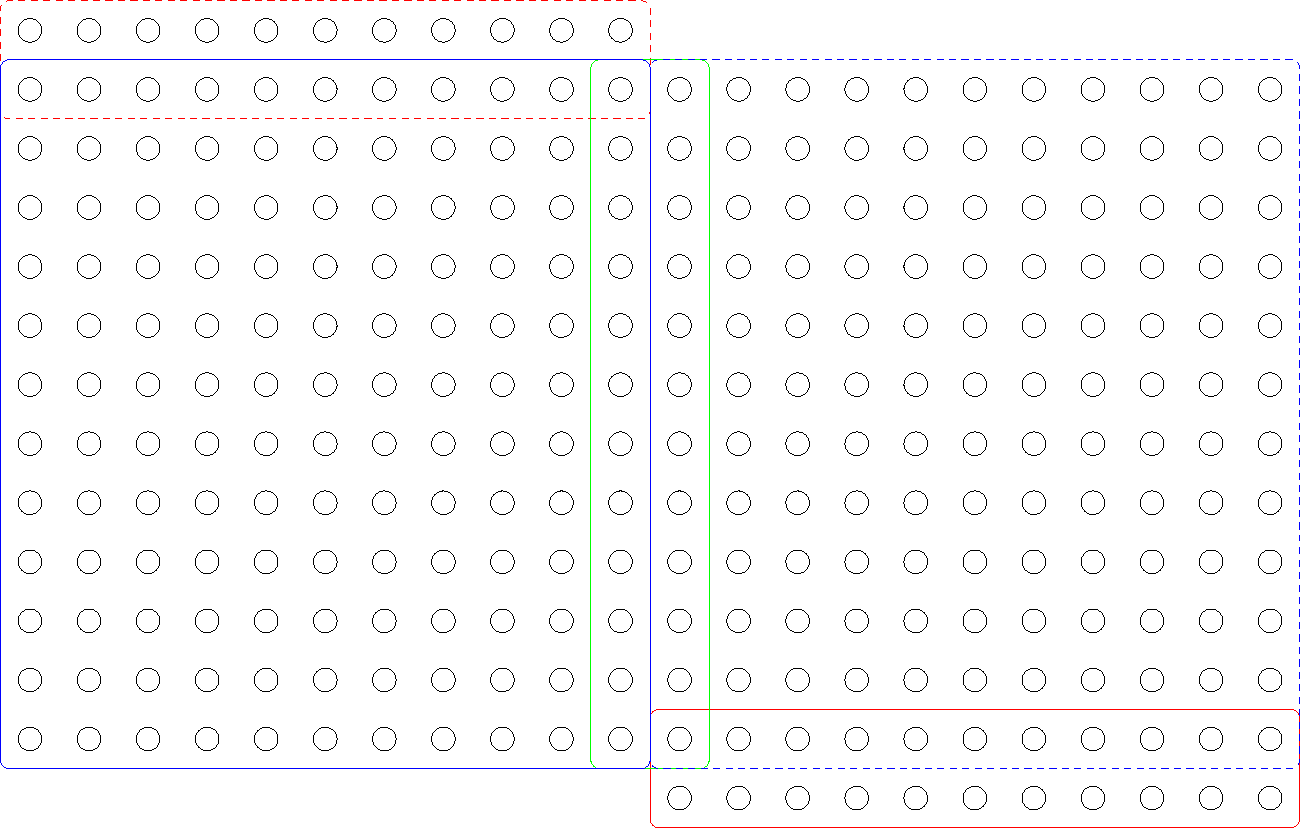
\includegraphics[width=0.6\textwidth]{figures/4/12x21x2_unfolded.pdf}
\caption{A proper unfolding of $G= (12,21,2)$. Colored rectangles indicate faces of $G$. Dashed lines indicate that cells appear on different layers. }
\label{fig:12x21x2_unfolded}
\end{figure} 

\begin{figure}[]
\centering
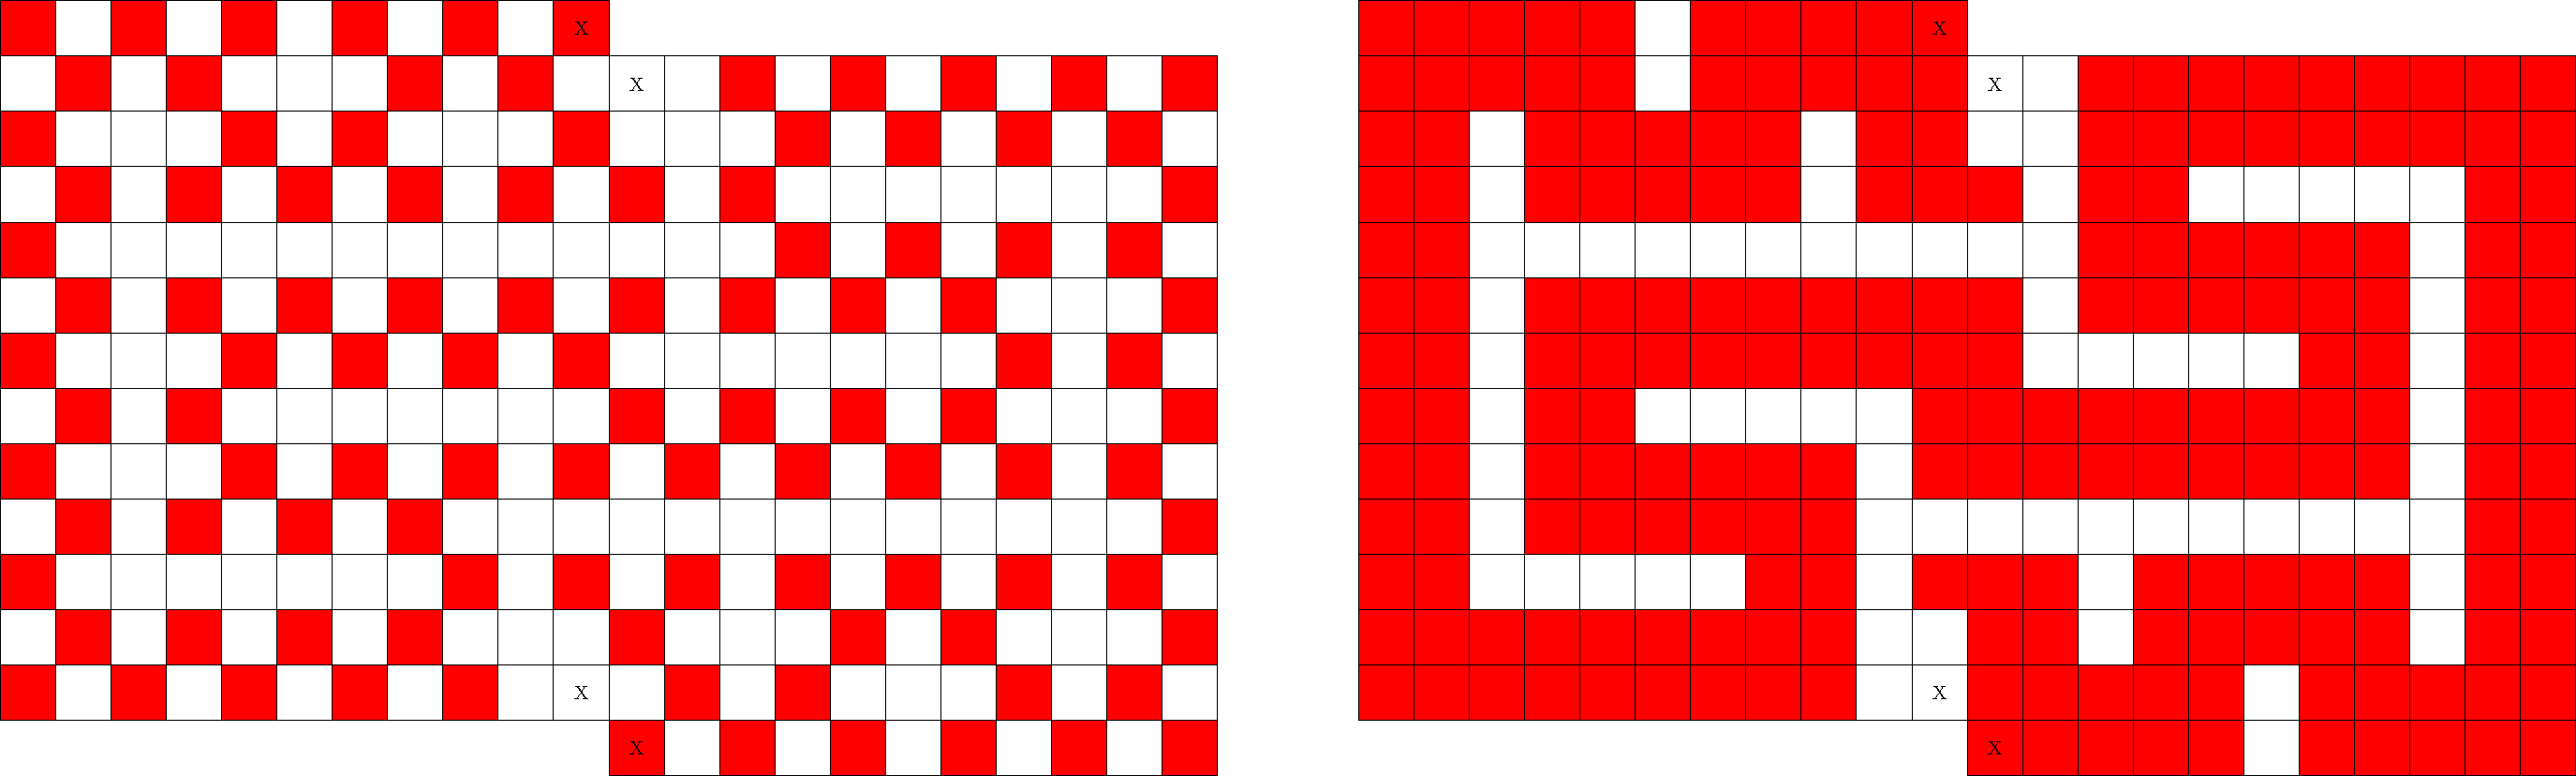
\includegraphics[width=0.8\textwidth]{figures/4/12x21x2_unfolded_lethal.pdf}
\caption{A percolating set on the proper unfolding of $G= (12,21,2)$.}
\label{fig:12x21x2_unfolded_lethal}
\end{figure} 

\section{Thickness 3}

\begin{con}
All $(a,b,3)$ grids $G$ with $a \equiv 3 \pmod 6$ and $b \equiv 1 \pmod 2$ are perfect. 
\end{con}

\begin{proof}
Consider the grid $H=(a+2,b+2,1)$, and observe that such a grid admits an optimal percolating set by construction \ref{con:snake}. Note that
$$\text{SA}(a,b,3) = \ceil{\text{SA}(a+2,b+2,1)} - 3.$$
We show that an unfolding of $G$ can be obtained from a simple augmentation of $H$. Let $H'$ be the grid obtained by deleting the four vertices in the bottom, right-most corner of $H$ (see figure \ref{fig:17x25x1_unfolded}). Consider the folding pattern illustrated in figure \ref{fig:17x25x1_manifold}, and observe that the pairs of vertices adjacent to the deleted region are duplicates of each other. (In other words, consider folding up the red and green regions in figure \ref{fig:17x25x1_manifold}, and notice that this operation causes vertices to overlap.) Taking this into account, the unfolding of $G$ percolates by lemma \ref{lem:forest}. Since $H$ admits an optimal percolating set of size $\ceil{\text{SA}(a+2,b+2,1)}$, and precisely 3 of the vertices deleted from $H$ to obtain $H'$ were infected, it follows that the unfolding of $G$ percolates at the lower bound. Finally, by lemma \ref{lem:three_walls}, since the unfolding of $G$ is proper and percolates at the lower bound, $G$ is perfect.
\end{proof}

\begin{figure}[]
\centering
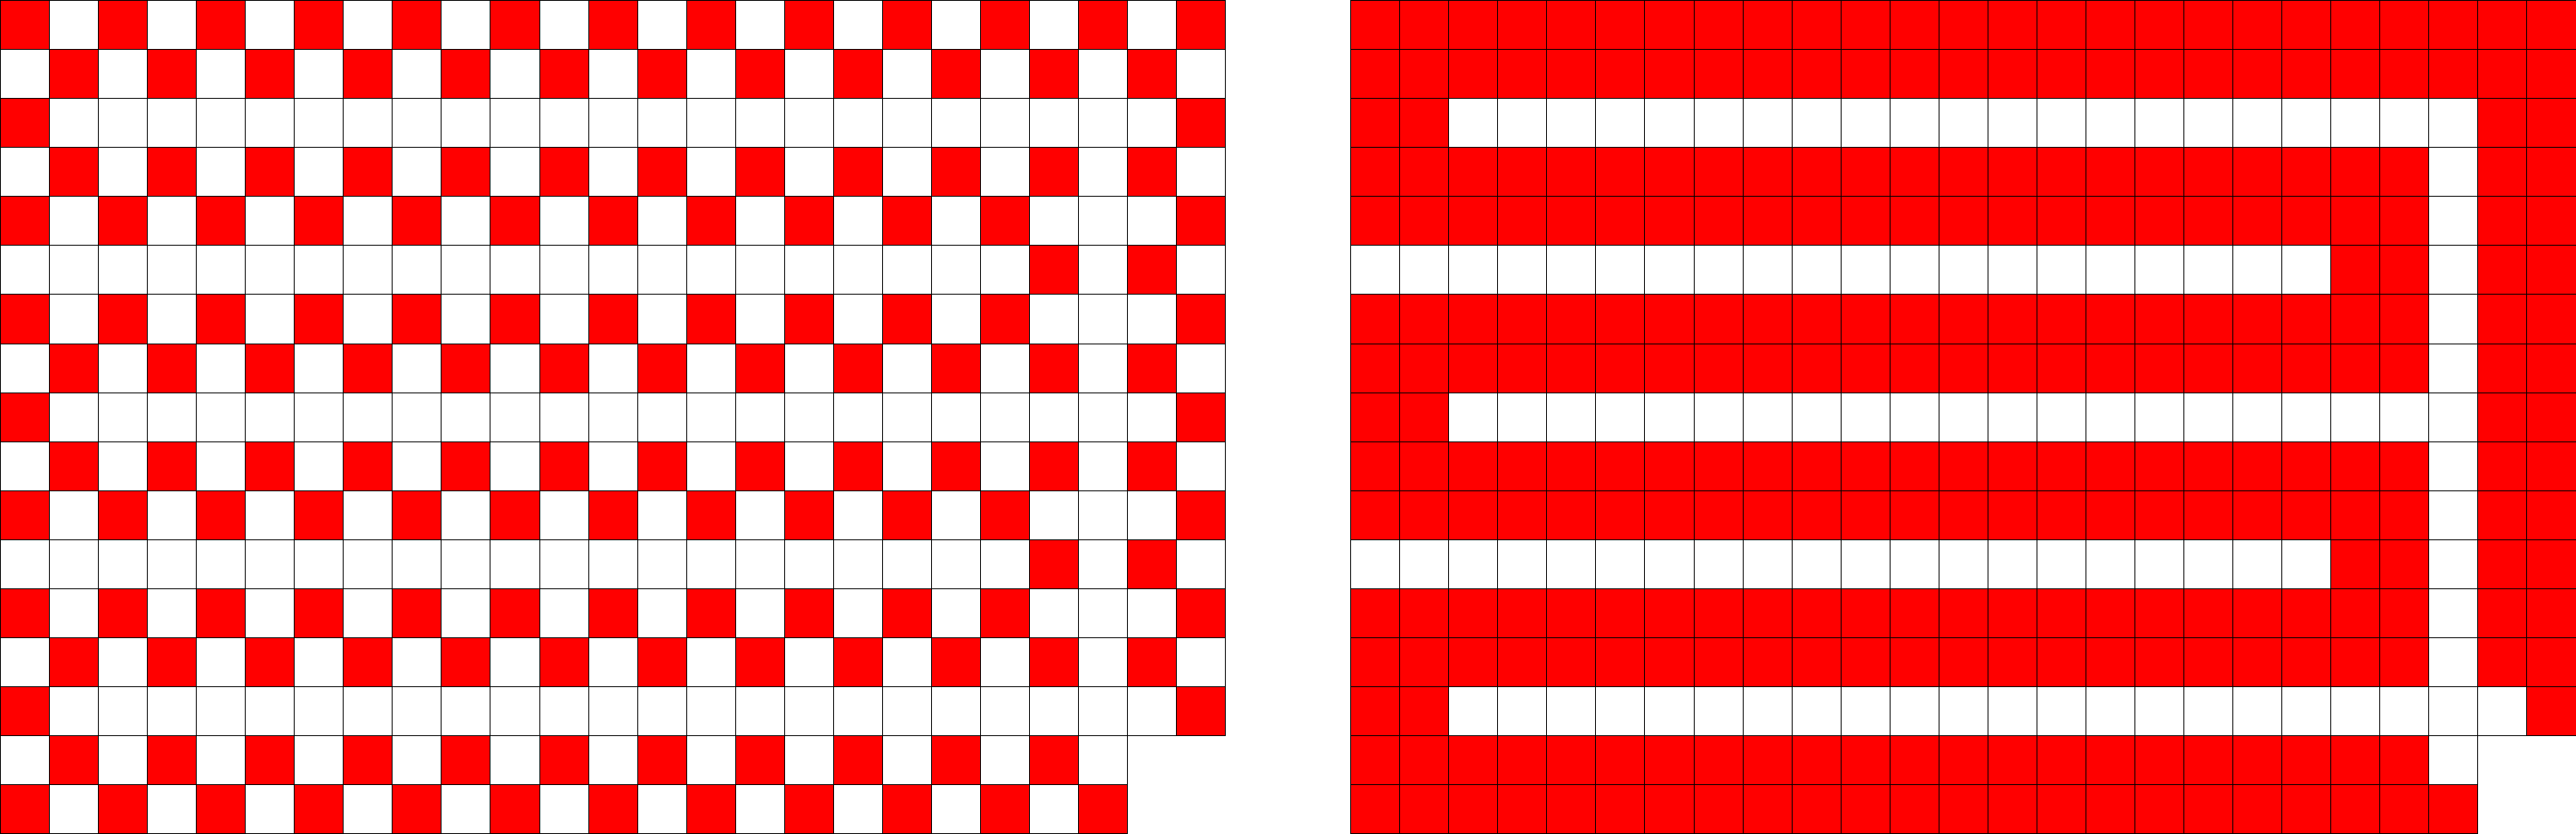
\includegraphics[width=0.8\textwidth]{figures/4/17x25x1_unfolded.pdf}
\caption{A percolating set on the proper unfolding $H'$ of $G= (15,23,3)$.}
\label{fig:17x25x1_unfolded}
\end{figure}

\begin{figure}[]
\centering
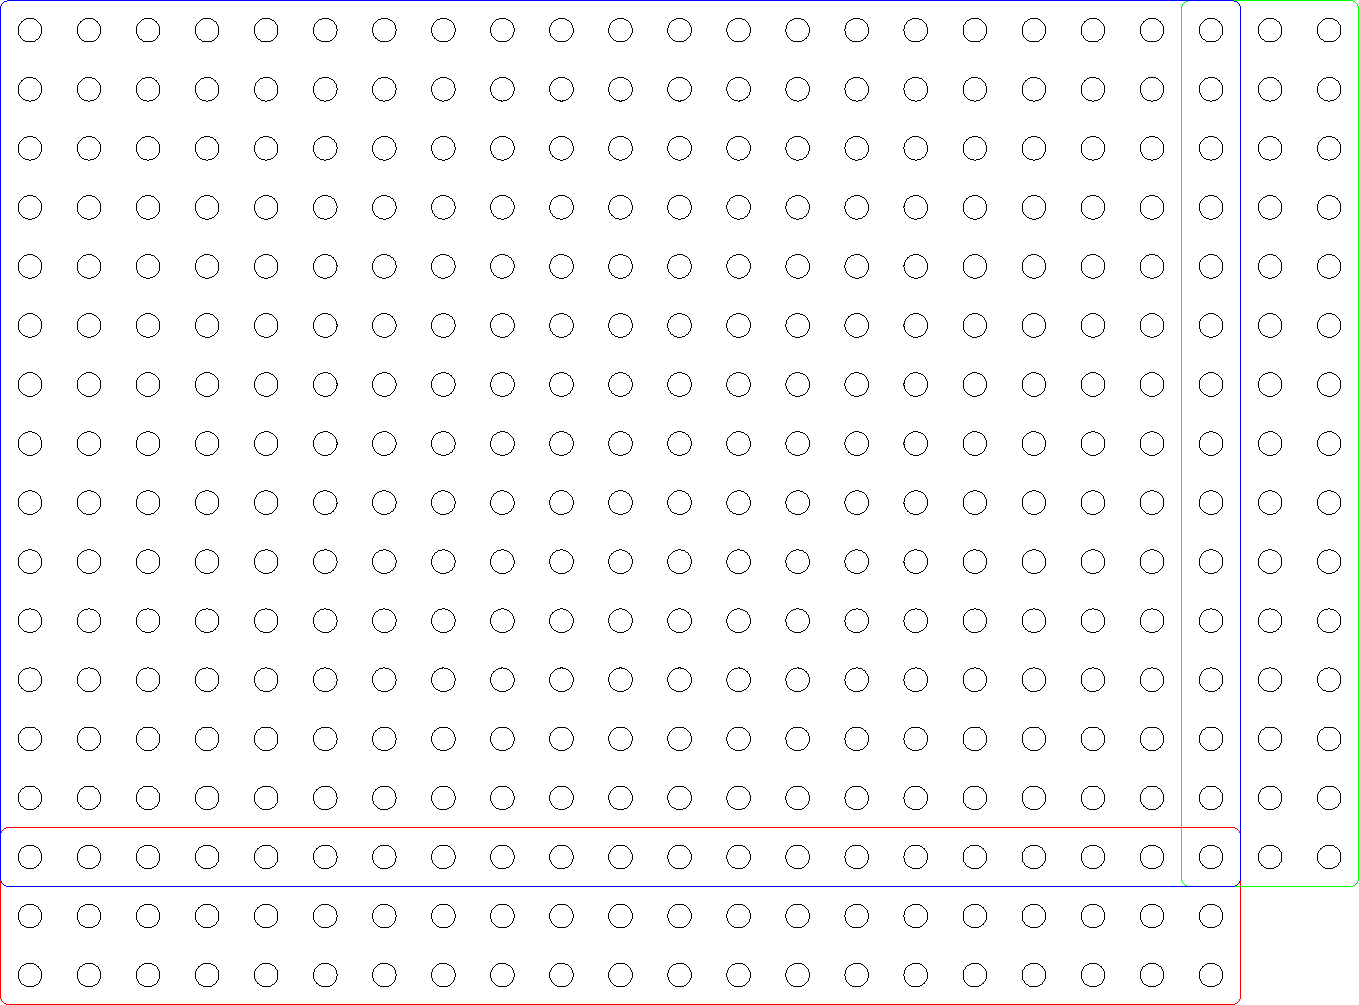
\includegraphics[width=0.6\textwidth]{figures/4/17x25x1_manifold.pdf}
\caption{A proper unfolding of $G= (15,23,3)$. Colored rectangles indicate faces of $G$. }
\label{fig:17x25x1_manifold}
\end{figure}

% (5, 3, 3)

% (5, 2, 2) 

% (5, 5, 5)

% (8, 5, 5)

% (a, 3, 3)

% (6, 3, 3)

% (6, 3, 2)

\begin{figure}[]
\centering
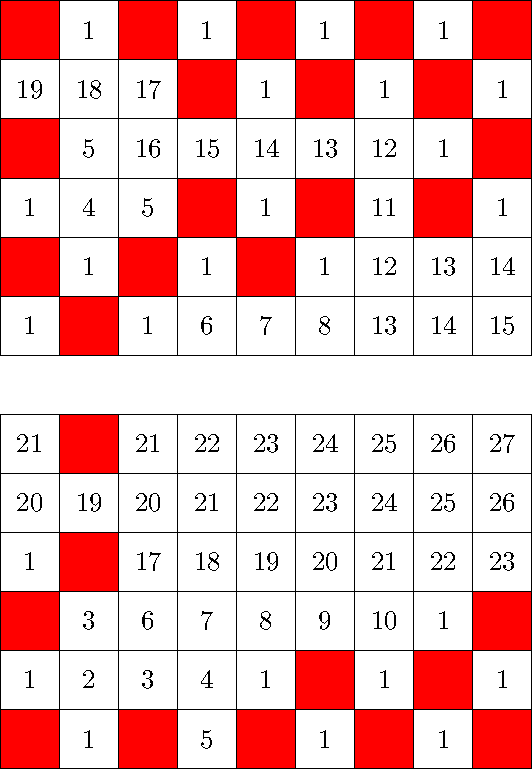
\includegraphics[width=\textwidth]{figures/4/6x9x2_numbered_heatmap.pdf}
\caption{}
\label{fig:6x9x2}
\end{figure} 

\begin{figure}[]
\centering
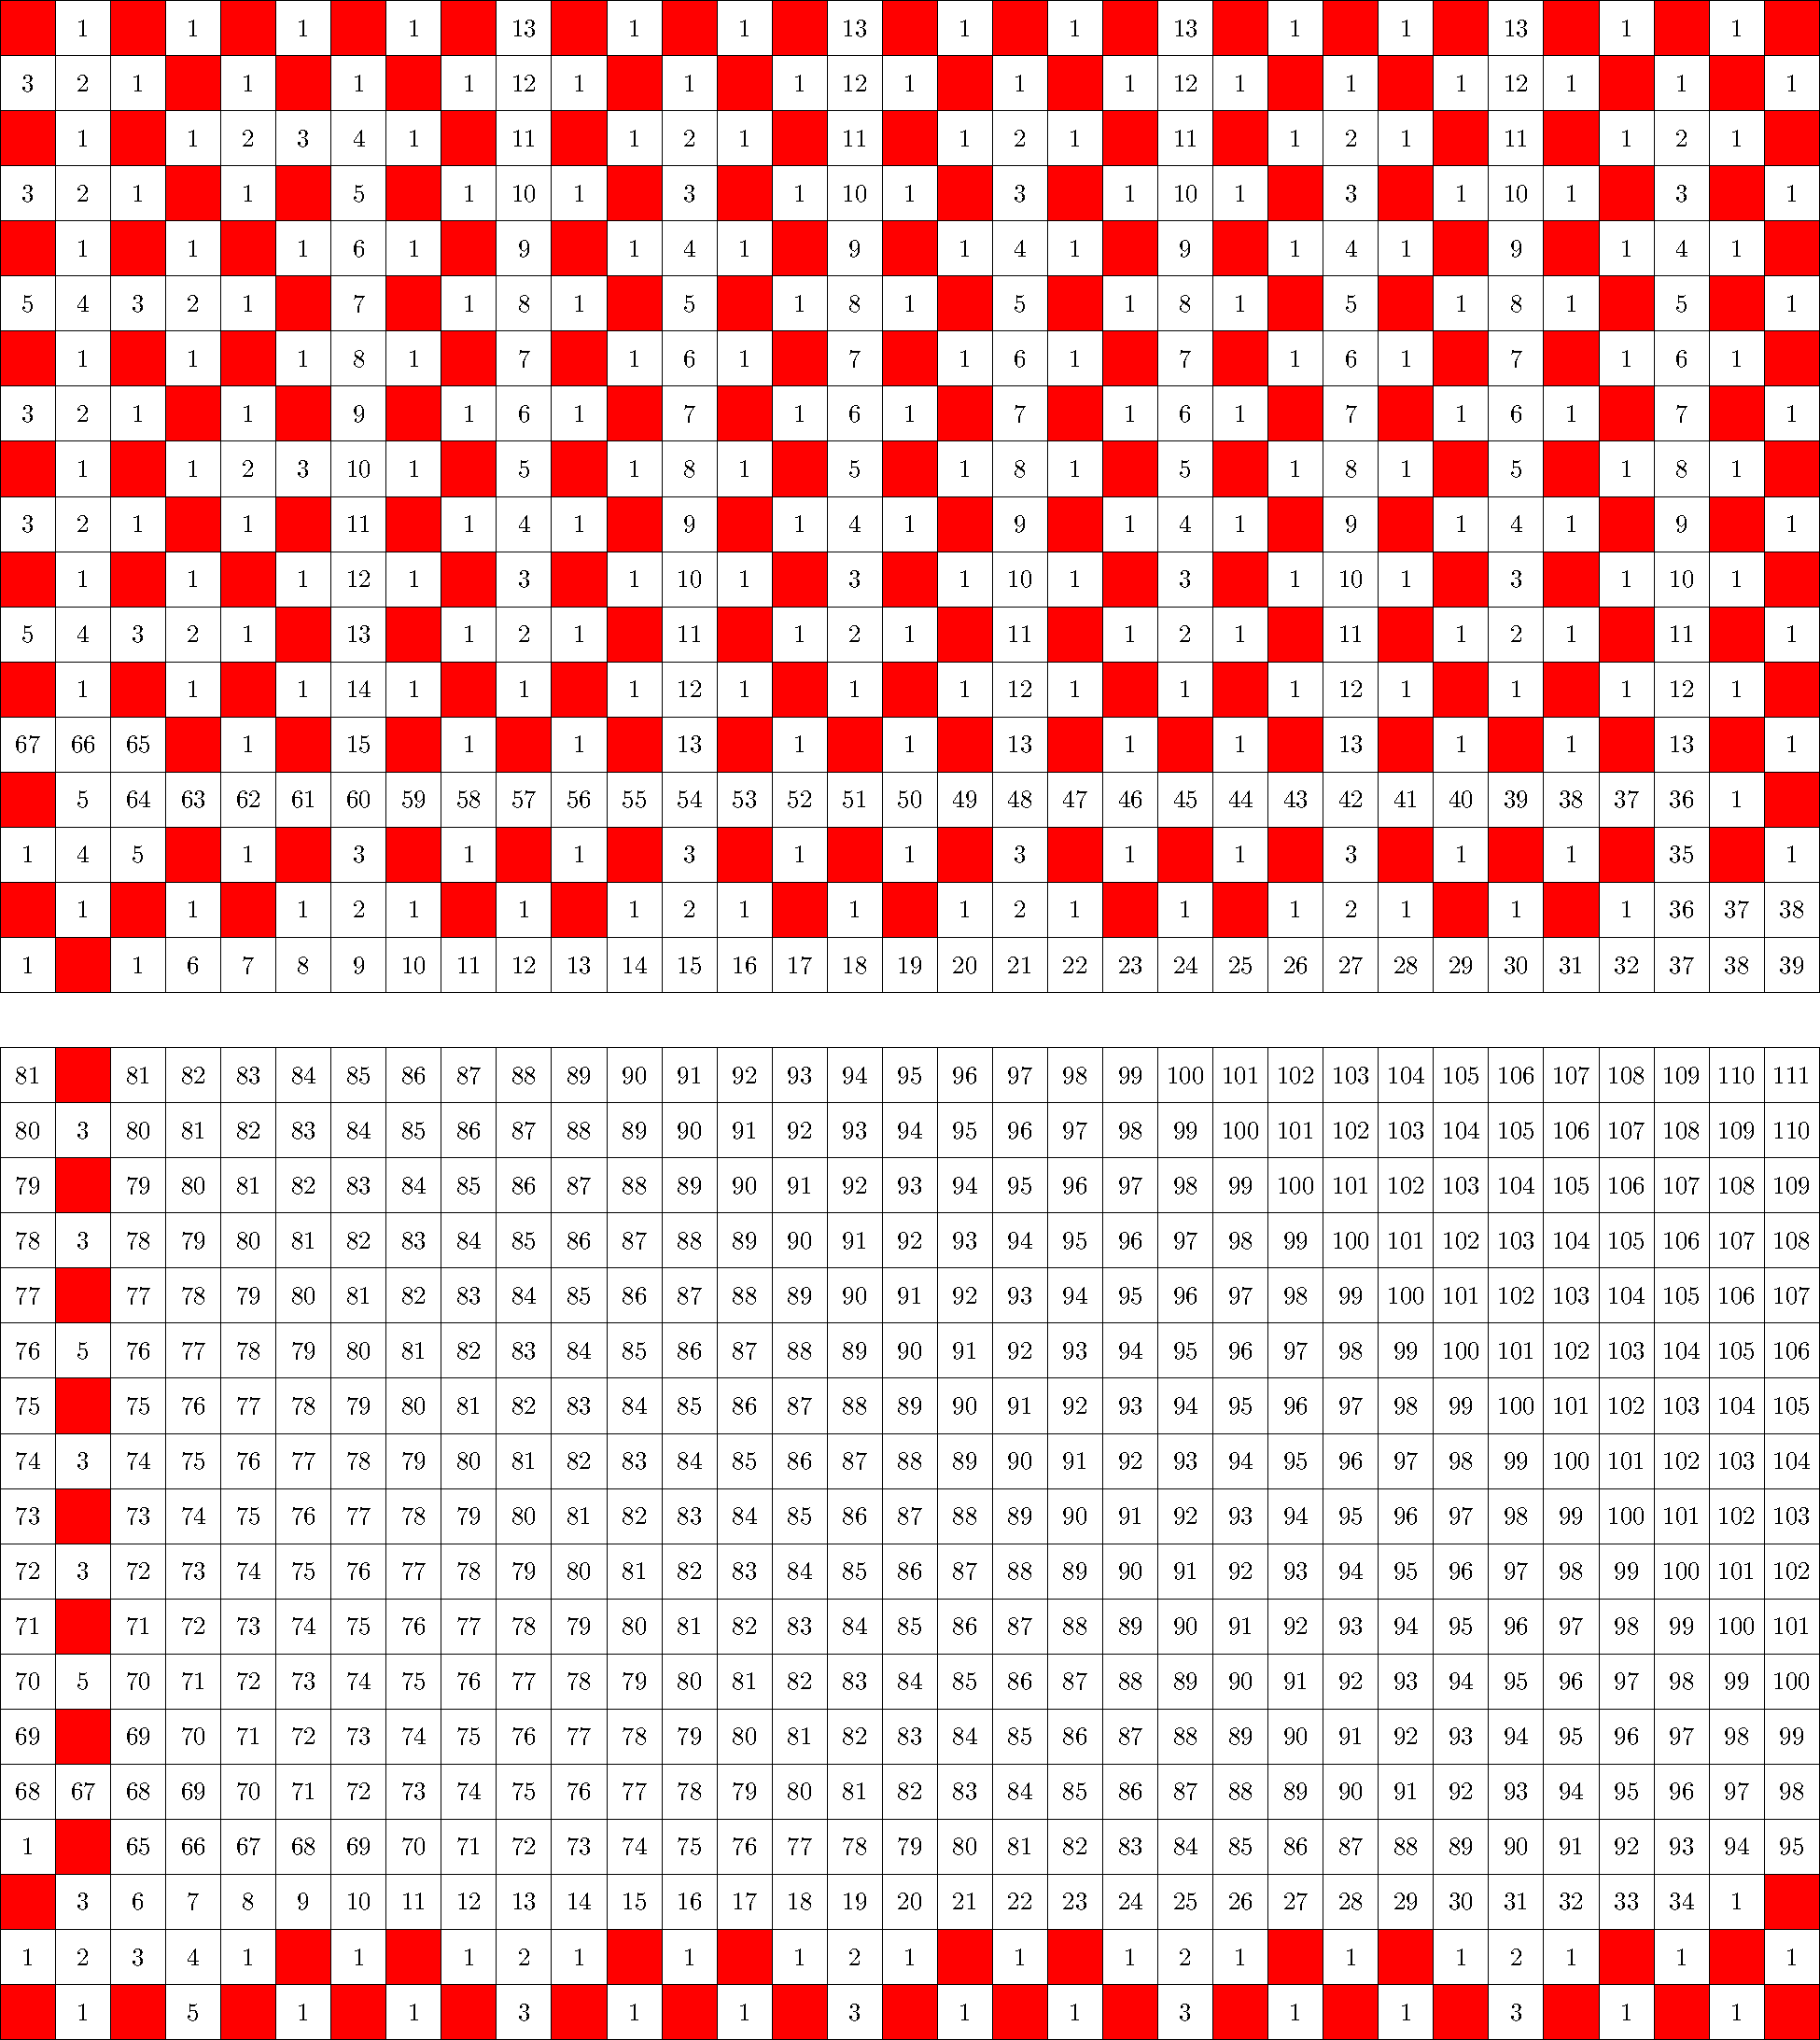
\includegraphics[width=\textwidth]{figures/4/18x33x2_numbered_heatmap.pdf}
\caption{}
\label{fig:6x9x2}
\end{figure} 

